Как было сказано выше, для разработки была выбрана пассивная BMS.
В качестве основного чипа был выбран TL-431. \\
Краткое описание:
Регулируемый источник опорного напряжения.
Используется для мониторинга напряжения на ячейке, сигнал выдаваемый схемой имеет нелинейную зависимость.

\begin{figure}[h]
    \centering
    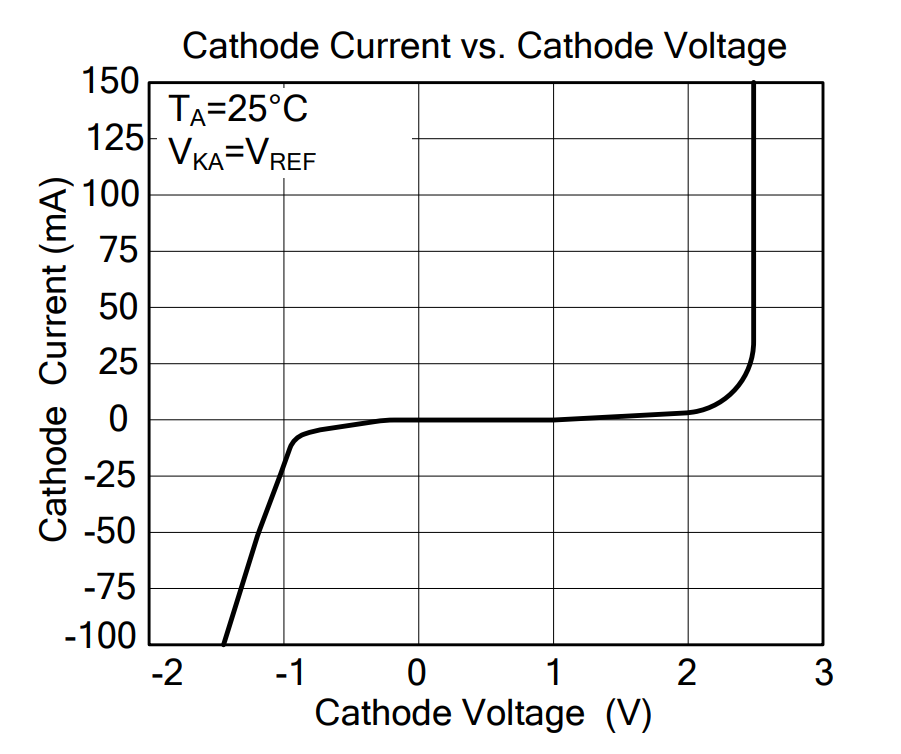
\includegraphics[width=0.55\linewidth]{img/tl431_graph_cathod_v_i.png}
    % \caption{принципиальная схема балансровки}
    \label{fig:tl431_curve_cathode_v_i}
\end{figure}


Ниже представлена принципиальная схема балансировки (см. \figurename  \ref{fig:principial})

\begin{figure}[p!]
    \centering
    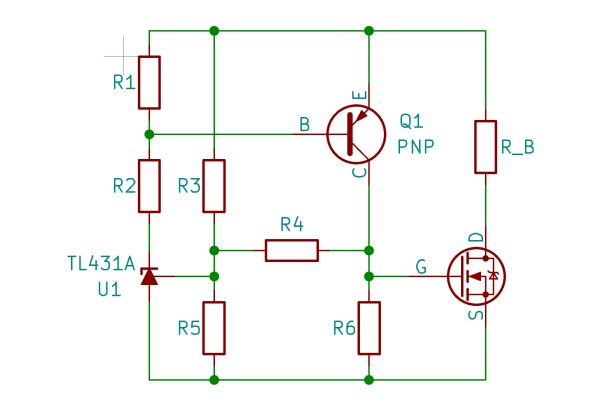
\includegraphics[width=0.9\linewidth]{img/principial.jpg}
    \caption{Принципиальная схема балансровки}
    \label{fig:principial}
\end{figure}

\subsubsection{Назначение компонентов принципиальной схемы}

1) Резисторы $R3$ и  $R5$  $-$ образуют делитель напряжения, 
который определяет напряжение начала балансировки(4.21В) 